\documentclass[border=10pt]{standalone}
\usepackage[T1]{fontenc}
\usepackage{helvet}
\renewcommand{\familydefault}{\sfdefault}
\usepackage{tikz}
\usetikzlibrary{arrows.meta,positioning,calc,decorations.pathreplacing,fit}

\definecolor{idpblue}{HTML}{005DAA}
\definecolor{idpcyan}{HTML}{00B3FF}
\definecolor{warm}{HTML}{D7263D}
\definecolor{inkgray}{HTML}{444444}
\definecolor{forestgreen}{HTML}{2E7D32}

\begin{document}
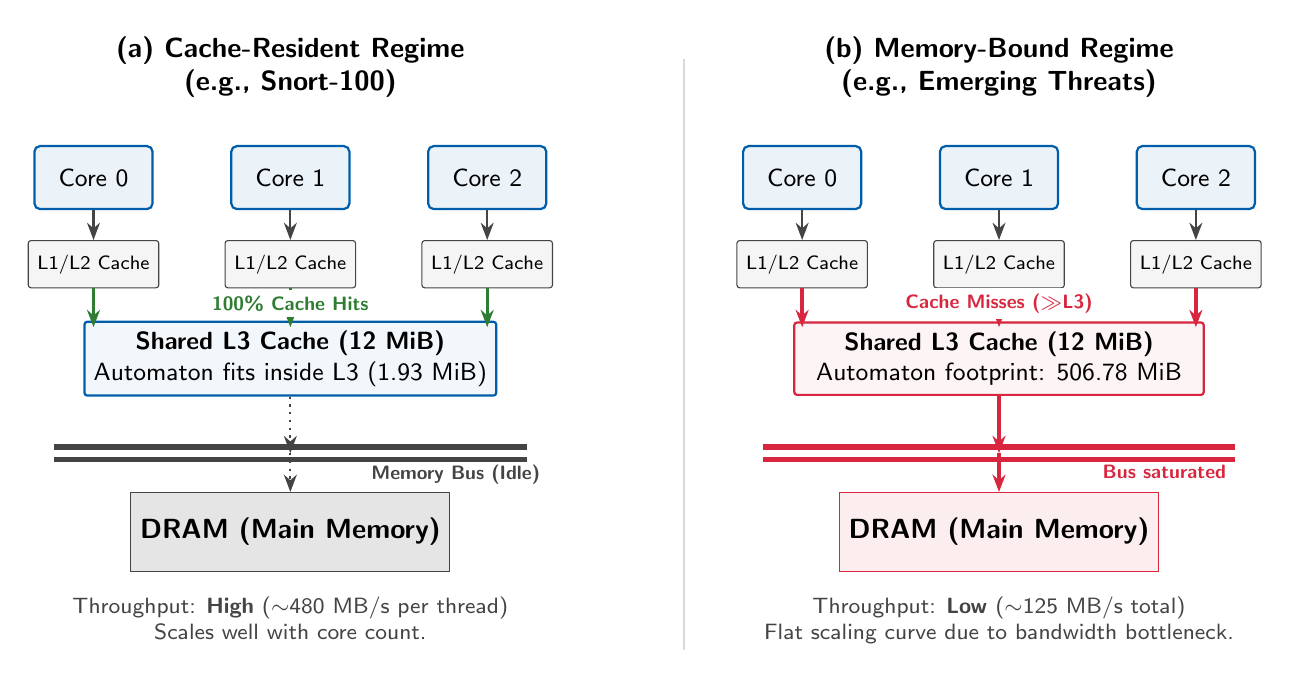
\begin{tikzpicture}[
    font=\small,
    >={Stealth[length=2.2mm]},
    title/.style={font=\bfseries},
    core/.style={draw=idpblue, fill=idpblue!8, thick, rounded corners=2pt, minimum width=15mm, minimum height=8mm, align=center},
    cache/.style={draw=inkgray, fill=gray!8, rounded corners=1pt, align=center},
    l12/.style={cache, minimum width=15mm, minimum height=6mm, font=\scriptsize},
    l3/.style={cache, draw=idpblue, fill=idpblue!5, thick, minimum width=52mm, minimum height=8mm},
    dram/.style={draw=inkgray, fill=gray!20, minimum width=30mm, minimum height=10mm, align=center, font=\bfseries},
    bus/.style={draw=inkgray, line width=2.0pt, double=white, double distance=2.5pt},
    arrow/.style={->, line width=0.8pt, draw=inkgray},
    hitarrow/.style={->, line width=1.2pt, draw=forestgreen},
    missarrow/.style={->, line width=1.5pt, draw=warm},
    note/.style={font=\footnotesize, text=inkgray, align=center},
]

    % =====================================================================
    % (a) CACHE-RESIDENT REGIME (Small Automaton)
    % =====================================================================
    \node[title, align=center] at (2.5, 4.4) {(a) Cache-Resident Regime\\(e.g., Snort-100)};
    
    % Cores
    \node[core] (c0) at (0, 3.0) {Core 0};
    \node[core] (c1) at (2.5, 3.0) {Core 1};
    \node[core] (c2) at (5.0, 3.0) {Core 2};
    
    % L1/L2 Caches
    \node[l12] (l2_0) at (0, 1.9) {L1/L2 Cache};
    \node[l12] (l2_1) at (2.5, 1.9) {L1/L2 Cache};
    \node[l12] (l2_2) at (5.0, 1.9) {L1/L2 Cache};
    
    \draw[arrow] (c0) -- (l2_0);
    \draw[arrow] (c1) -- (l2_1);
    \draw[arrow] (c2) -- (l2_2);
    
    % Shared L3 Cache
    \node[l3] (l3_a) at (2.5, 0.7) {\textbf{Shared L3 Cache (12 MiB)}\\Automaton fits inside L3 (1.93 MiB)};
    
    \draw[hitarrow] (l2_0) -- (0, 1.1);
    \draw[hitarrow] (l2_1) -- (2.5, 1.1);
    \draw[hitarrow] (l2_2) -- (5.0, 1.1);
    \node[forestgreen, font=\scriptsize\bfseries, fill=white, inner sep=2pt] at (2.5, 1.4) {100\% Cache Hits};

    % DRAM & Bus (Unused/idle)
    \draw[bus] (-0.5, -0.5) -- (5.5, -0.5) node[pos=0.85, below, font=\scriptsize\bfseries, text=inkgray] {Memory Bus (Idle)};
    \node[dram] (dram_a) at (2.5, -1.5) {DRAM (Main Memory)};
    
    \draw[arrow, dotted] (l3_a.south) -- (2.5, -0.5);
    \draw[arrow, dotted] (2.5, -0.5) -- (dram_a.north);
    
    \node[note, anchor=north] at (2.5, -2.2) {Throughput: \textbf{High} ($\sim$480 MB/s per thread)\\Scales well with core count.};

    % =====================================================================
    % (b) MEMORY-BOUND REGIME (Large Automaton)
    % =====================================================================
    \begin{scope}[xshift=9.0cm]
        \node[title, align=center] at (2.5, 4.4) {(b) Memory-Bound Regime\\(e.g., Emerging Threats)};
        
        % Cores
        \node[core] (c0_b) at (0, 3.0) {Core 0};
        \node[core] (c1_b) at (2.5, 3.0) {Core 1};
        \node[core] (c2_b) at (5.0, 3.0) {Core 2};
        
        % L1/L2 Caches
        \node[l12] (l2_0_b) at (0, 1.9) {L1/L2 Cache};
        \node[l12] (l2_1_b) at (2.5, 1.9) {L1/L2 Cache};
        \node[l12] (l2_2_b) at (5.0, 1.9) {L1/L2 Cache};
        
        \draw[arrow] (c0_b) -- (l2_0_b);
        \draw[arrow] (c1_b) -- (l2_1_b);
        \draw[arrow] (c2_b) -- (l2_2_b);
        
        % Shared L3 Cache
        \node[l3, draw=warm, fill=warm!5] (l3_b) at (2.5, 0.7) {\textbf{Shared L3 Cache (12 MiB)}\\Automaton footprint: 506.78 MiB};
        
        % Cache Misses
        \draw[missarrow] (l2_0_b) -- (0, 1.1);
        \draw[missarrow] (l2_1_b) -- (2.5, 1.1);
        \draw[missarrow] (l2_2_b) -- (5.0, 1.1);
        \node[warm, font=\scriptsize\bfseries, fill=white, inner sep=2pt] at (2.5, 1.4) {Cache Misses ($\gg$L3)};
        
        % Bus & DRAM (Saturated)
        \draw[bus, draw=warm] (-0.5, -0.5) -- (5.5, -0.5) node[pos=0.85, below, font=\scriptsize\bfseries, text=warm] {Bus saturated};
        \node[dram, draw=warm, fill=warm!8] (dram_b) at (2.5, -1.5) {DRAM (Main Memory)};
        
        \draw[missarrow] (l3_b.south) -- (2.5, -0.5);
        \draw[missarrow] (2.5, -0.5) -- (dram_b.north);
        
        \node[note, anchor=north] at (2.5, -2.2) {Throughput: \textbf{Low} ($\sim$125 MB/s total)\\Flat scaling curve due to bandwidth bottleneck.};
    \end{scope}
    
    % Divider
    \draw[gray!30, line width=0.5pt] (7.5, 4.5) -- (7.5, -3.0);

\end{tikzpicture}
\end{document}
